%
% main.tex -- Paper zum Thema komplexe Morlet Wavelets und CWT
%
% (c) 2019 Hochschule Rapperswil
%

\chapter{Komplexe Wavelets und CWT\label{chapter:complex}}
\lhead{Komplexe Wavelets und CWT}
\begin{refsection}
\chapterauthor{Roy Seitz}

% \section{Einleitung}
Die diskrete Wavelet-Transformation (DWT) mit reellen Wavelets ist besonders schnell zu berechnen.
Deshalb ist sie die bevorzugte Wahl zur Signalverarbeitung.
Beim Erstellen `schöner' Bilder trifft man jedoch unter Anderem auf folgende drei Probleme:

Erstens wäre es für Bilder vorteilhaft, die relevanten Frequenzpunkte vorgeben zu können.
So kann man direkt lineare oder logarithmische Skalen wählen. Die DFT ist an Zweierpotenzen gebunden. %TODO: Referenz zum Frame für a^n statt 2^n
Zweitens erfordern die meisten Methoden zum Erstellen von Bildern ein reguläres Raster.
Die DFT liefert aber in jeder zusätzlichen Zeile nur noch halb so viele Punkte.
Drittens, wenn man Schwingungen finden möchte, ist es vorteilhaft, wenn die Amplitude ersichtlich ist.
Sie kann beispielsweise als Helligkeit abgebildet werden. 
Bei reellen Wavelets sind Amplitude und Phase jedoch nicht einfach zu trennen.

Die CWT aus Kapitel~\ref{chapter:cwt} ist die bevorzugte Wahl für analytische Berechnungen.
Als kontinuierliche Transformation benötigt sie jedoch etwas Vorarbeit,
nämlich eine Diskretisierung der $a$- und $b$-Variablen.
Eine anschliessende direkte Berechnung der diskretisierten Integrale ist allerdings sehr rechenintensiv.
Im ersten Abschnitt betrachten wir deshalb, wie man die CWT als Faltung interpretieren kann, welche sich effizient mittels FFT berechnen lässt.
Zur Illustration verwenden wir ein einfaches Beispielsignal und die CWT mittels Haar-Wavelet.

Die Wahl des Wavelets spielt eine zentrale Rolle und beeinflusst das erhaltene Bild wesentlich.
Ein wichtiger Punkt ist hierbei die Unschärfe-Relation zwischen Zeit und Frequenz.
Ein Signal kann nicht in beidem zugleich gut lokalisiert sein.
Im zweiten Abschnitt vergleichen wir deshalb die CWT mittels Haar- und Gabor-Wavelet anhand zweier Beispielsignale.

Im dritten Abschnitt wenden wir uns den komplexen Wavelets zu.
Via Hilbert-Transformation können wir basierend auf einem beliebigen Wavelet ein neues finden, bei welchem sich Phasen und Amplitude trennen lassen.

Durch die Berechnung der CWT mittels FFT entstehen Artefakte durch die zirkuläre Faltung.
Geschickte Erweiterung des Signals kann diesen Effekt vermeiden.
Dies beeinflusst jedoch massgeblich die Performance, da durch Erweitern des Signals der Rechenaufwand signifikant steigt.
Im letzten Abschnitt vergleichen wir deshalb den Rechenaufwand und die erzielten Bilder mit verschiedenen Padding-Optionen anhand eines Matlab-Skripts.
Zudem vergleichen wir die Performance dieses Skripts mit der Implementation von Matlab selbst.
Überraschenderweise ist es auf den getesteten Rechnern in jedem Fall schneller als die cwt-Funktion aus der Wavelet-Toolbox von Matlab.

%%%%%%%%%%%%%%%%%%%%%%%%%%%%%%%%%%%%%%%%%%%%%%%
\section{Effiziente Berechnung der CWT}
\rhead{Berechnung der CWT}
Als erstes möchten wir herausfinden, wie sich die CWT effizient berechnen lässt.
Als zweites werden wir zwei Beispielsignale definieren und die CWT mittels Haar-Wavelet betrachten.
Abschliessend rechnen wir die CWT noch mit dem Gabor-Wavelet und vergleichen die beiden Bilder.

\subsection{CWT als Faltung}
Betrachten wir zuerst die folgende Gleichung
\begin{equation}
\Wave f (a,b)
=
\langle f,\psi_{a,b}\rangle
=
\frac{1}{\sqrt{|a|}}\int_{-\infty}^\infty f(t)\,
	\overline{\psi}\biggl(\frac{t-b}{a}\biggr)\,dt,\label{complex:CWT}
\end{equation}
durch welche in Definition~\ref{cwt:definition} die kontinuierliche Wavelet-Transformation eingeführt wurde.
Dieses Integral entspricht der Faltung zwischen $f(t)$ und 
\begin{equation} 
    g(t) 
    = \frac{1}{\sqrt{|a|}} \overline\psi\biggl(\frac{-t}{a}\biggr).
\end{equation}
Der Standard-Trick zur effizienten Berechnung einer Faltung ist die Multiplikation im Frequenzbereich.
\begin{equation} 
\mathcal{W}f (a,b) = (f*g)(t) = \mathcal{F}^{-1}\biggl\lbrace\hat f(\omega) \hat g (\omega) \biggr\rbrace.
\end{equation}
Dafür benötigen wir die Fouriertransformierte $\hat g (\omega)$:
\begin{align*}
	\hat g (\omega) = 
    \Four\,\biggl\lbrace \frac{1}{\sqrt{|a|}} \overline\psi \biggl(\frac{-t}{a}\biggr) \biggr\rbrace 
	&= \frac{1}{\sqrt{|a|}} \int_{-\infty}^{\infty}\overline\psi\biggl(\frac{-t}{a}\biggr) \, e^{-i\omega t}\,dt\\
	&= \frac{1}{\sqrt{|a|}} \overline{\int_{-\infty}^{\infty}\psi \biggl(\frac{-t}{a}\biggr) \, e^{i\omega t}\,dt}  
    & \biggl(\text{Substitution } t' = \frac{-t}{a}\biggr)\\
	&= \frac{1}{\sqrt{|a|}} \overline{\int_{-\infty}^{\infty}\psi(t') \, e^{-ia\omega t'} |a|\,dt'}\\
	&= \sqrt{|a|} \, \overline{\hat{\psi}}(a\omega).
\end{align*}
Gleichung~\eqref{complex:CWT} lässt sich somit schreiben als
\begin{equation}
\Wave f(a,b)
= \mathcal{F}^{-1}\bigl\lbrace\hat{f}(\omega) \sqrt{|a|}\, \overline{\hat{\psi}}(a\omega)\bigr\rbrace. \label{complex:fcwt}
\end{equation}

Mittels Fourier-Transformation lässt sich die Wavelet-Transformation folglich besonders elegant berechnen.
Kontinuierliche Funktionen sind für numerische Systeme jedoch ungeeignet.
Die CWT muss in $a$ und $b$ diskretisiert werden.
Die Diskretisierung von $b$ entspricht vorteilhaft gerade derjenigen des Signals selbst.
Dann lässt sich die Fourier-Transformation mittels FFT effizient berechnen und Gleichung~\eqref{complex:fcwt} wird zu
\begin{equation}
	\mathcal{W}f(a,b) = \text{IFFT}\bigl(\text{FFT}(f) \, \overline{\hat{\psi}}(a\omega)\bigr). \label{complex:ffcwt}
\end{equation}

Der Faktor $\sqrt{|a|}$ wurde hierbei weggelassen.
Hierdurch werden die hohen Frequenzen stärker gewichtet und $|\!\Wave f(a,b)|$ ist gerade proportional zur Amplitude der analysierten Signalkomponente.
Zudem erzielen wir im Diskreten nicht exakt die Faltung, sondern die zirkuläre Version davon. 
Mehr dazu im Abschnitt~\ref{complex:circ-conv-padding}.

Gleichung~\eqref{complex:ffcwt} muss für jedes $a$ einzeln gelöst werden.
Sie wird besonders interessant, wenn das Wavelet im Frequenzbereich eine geschlossene, analytische Form besitzt.
Dann benötigt man nur eine FFT für das Signal, so wie für jedes $a$ eine inverse FFT und eine punktweise Multiplikation zwischen Signal und Wavelet.

%\clearpage
\subsection{Das Haar-Wavelet}
\rhead{Haar-Wavelet}
\begin{figure}
	\centering
	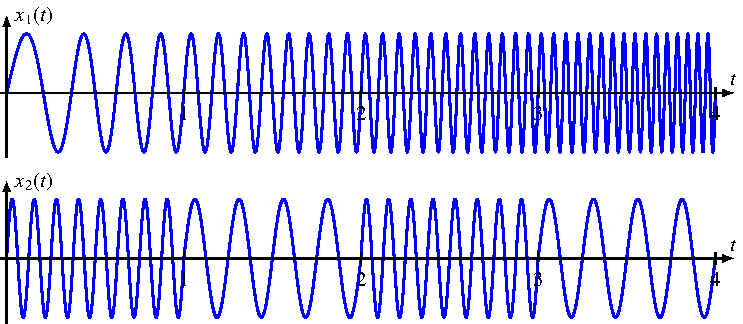
\includegraphics{papers/complex/images/signals.pdf}
	\caption{Die beiden Beispielsignale $x_1(t)$ und $x_2(t)$}
\end{figure}
Rechnen wir das erste Beispiel.
Hierfür benötigen wir zwei Dinge: Signal und Wavelet.
Als Signale nehmen wir zwei Sinus-Schwingungen, eine mit linear ansteigender und eine mit stückweise konstanter Frequenz.
\begin{align}
    x_1(t) &= \sin\left( \int_{0}^{t} 2\pi f_1(\tau)\,d\tau\right) & f_1(t) &= 2 + 6/4 \cdot t \\
    x_2(t) &= \sin\left( \int_{0}^{t} 2\pi f_2(\tau)\,d\tau\right) & f_2(t) &= \left\lbrace \begin{matrix}
    4, & &t& < 1\\
    8, & 1.0 \le &t& < 2.0\\
    4, & 2.0 \le &t& < 3.0\\
    8, & 3.0 \le &t&\\
    \end{matrix}\right.
\end{align}
Das Haar-Wavelet sei in diesem Abschnitt zentriert um $t=0$.
Die daraus resultierende Symmetrie wird sich in der Berechnung der Fourier-Transformation als hilfreich erweisen.

\begin{definition}
	\label{complex:def-haar-wavelet}
	Das Haar-Wavelet besitzt folgende Gestalt:
	\[
	\psi_{\text{Haar}}(t) = \left\lbrace\begin{matrix*}[r]
	1 & -\frac{1}{2} \le t < 0  \\
	-1 & 0 \le t < \frac{1}{2} \\
	0 & \text{sonst}.
	\end{matrix*} \right.\label{complex:def-haar}
	\]
\end{definition}
Die Fourier-Transformierte von $\psi_{\text{Haar}}$ berechnet sich wie folgt:
\begin{align}
	\Four \psi_\text{Haar}  
	&= \frac{1}{\sqrt{2\pi}}\int_{-\infty}^{\infty} \psi_\text{Haar} e^{-i\omega t} \,dt\nonumber\\
	&= \frac{1}{\sqrt{2\pi}}\Biggl( \int_{-1/2}^{0} e^{-i\omega t} \,dt - \int_{0}^{1/2} e^{-i\omega t}\,dt \Biggr) \nonumber\\
	&= \frac{i}{\sqrt{2\pi}\omega}\bigl( \bigl[ e^{-i\omega t}\bigr]_{-1/2}^0  - \bigl[ e^{-i\omega t}\bigr]_{0}^{1/2} \bigr)\nonumber\\
	&= \frac{i}{\sqrt{2\pi}} \frac{1-\cos(\omega/2)}{\omega/2}\label{complex:f-psi-haar}
\end{align}
Das Haar-Wavelet ist also nicht nur im Zeit-, sondern auch im Frequenzbereich besonders einfach.
Insbesondere lässt sich die mit $a$ skalierte Version des Wavelets durch Satz~\ref{four-int:trans-dial} direkt im Frequenzbereich berechnen.
Abbildung~\ref{complex:haar} zeigt das Haar-Wavelet im Zeit- und Frequenzbereich.
Auffallend ist, dass das im Zeitbereich besonders gut lokalisierte Haar-Wavelet in der Frequenz sehr schlecht lokalisiert ist.
\begin{figure}
	\centering
	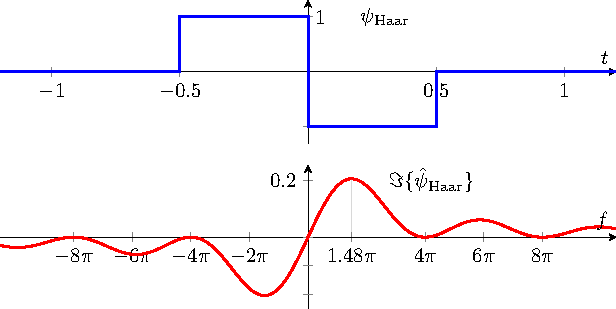
\includegraphics{papers/complex/images/haar.pdf}
	\caption{Das Haar-Wavelet}
	\label{complex:haar}
\end{figure}

\begin{figure}
	\centering
	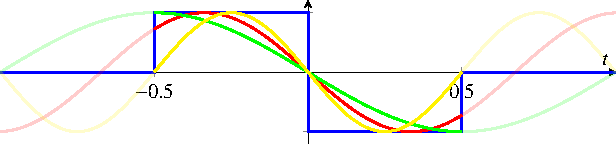
\includegraphics{papers/complex/images/haar_dom.pdf}
	
	\caption{Blau: $\psi_\text{Haar}$, Rot: $\sin ({\color{red}\omega_\psi}\cdot t)$, Gelb: $\sin ({\color{yellow}1.0}\cdot 2\pi t)$, Grün: $\sin ({\color{green}0.5}\cdot 2\pi t)$}
	\label{complex:dom-freq}
\end{figure}
An dieser Stelle definieren wir noch die \emph{dominante Frequenz} eines Wavelets.
\index{dominante Frequenz}%
\begin{definition}
	Die Fourier-Transformierte eines Wavelets erreicht den maximalen Betrag bei der \emph{dominanten Frequenz $\omega_\psi$}.
	\begin{equation}
		\omega_\psi \coloneqq \underset{\omega}{\text{\emph{argmax}}} \, |\hat\psi(\omega)|
	\end{equation}
	
\end{definition}

Die dominante Frequenz erlaubt, die $a$-Achse der Wavelet-Transformation als Frequenz-Achse zu interpretieren.
Für die Momentanfrequenz gilt
\[
	\omega(b) \approx \frac{\omega_\psi}{a_\text{max}(b)},
	\qquad 
	a_\text{max}(b)
	= 
	\underset{a}{\text{argmax}} \, |\!\Wave f(a,b)|.
\]
Diese Interpretation ist natürlich nur zulässig, wenn das Signal zum betrachteten Zeitpunkt nur eine dominante Frequenz-Komponente beinhaltet.
Bei unseren Beispielsignalen ist dies der Fall.
Abbildung~\ref{complex:dom-freq} illustriert die Bedeutung von $\omega_\psi$ für das Haar-Wavelet.
Es ist die Frequenz, bei welcher das Skalarprodukt mit dem Wavelet maximal wird.

Somit haben wir für unser Beispiel alles zusammen.
Nach einer Diskretisierung der Variablen überlassen wir die Arbeit dem Computer.
Dies liefert die Bilder aus Abbildung~\ref{complex:haar-ex}.

\begin{figure}
	\centering
	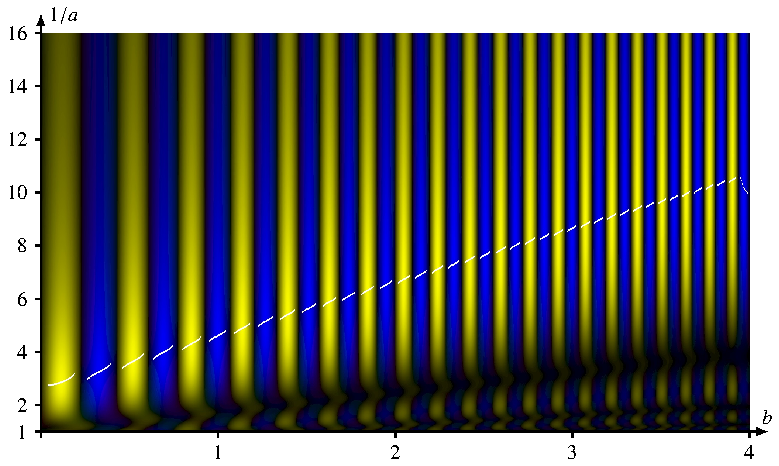
\includegraphics{papers/complex/images/chirp_haar.pdf}
	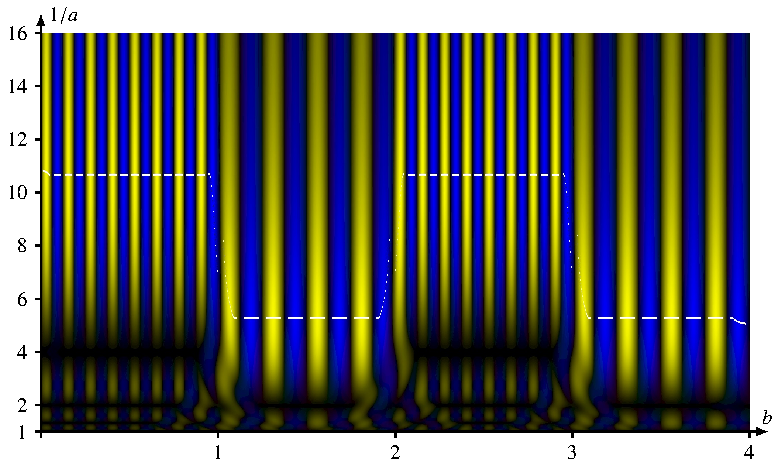
\includegraphics{papers/complex/images/square_haar.pdf}
	\caption{Wavelet-Transformationen der beiden Beispielsignale mit dem Haar-Wavelet. 
		Die Lokalisierung in der Zeit ist sehr gut, aber die momentane Frequenz ist kaum ersichtlich. 
		Zudem resultiert das periodische Signal in einer periodischen Helligkeit. 
		(Zur Erinnerung: bei reellen Werten entspricht die Farbe dem Vorzeichen, Blau: $+$, Gelb $-$)
	}
	\label{complex:haar-ex}
\end{figure}

Wie erwartet ist die Lokalisierung in der Frequenz ziemlich schlecht.
Das Haar-Wavelet gibt den Zeitpunkt einer Änderung der Frequenz zwar sehr genau wieder, die Frequenz selbst ist jedoch kaum ablesbar.
Als Orientierungshilfe sind $a_\text{max} (b) = \max_a{|\!\Wave x_n(a,b)|}$ weiss hervorgehoben.
Sie weichen um $\omega_\psi$ von der Signal-Frequenz ab, welche als Schwingung in der Amplitude gut erkennbar ist.
Dieses An- und Abschwellen des Betrags der Skalarprodukte verhindert es, $a_\text{max}(b)$ einfach zu folgen.
Dies werden wir im Abschnitt~\ref{complex:separate} durch komplexe Wavelets beheben.
Zuerst kümmern wir uns aber um die Lokalisierung in der Frequenz.

\documentclass[tikz]{standalone}
\usepackage{amsmath}
\usepackage{pgfplots}
\usepackage{csvsimple}

\usetikzlibrary{arrows,intersections,math}

\begin{document}
\begin{tikzpicture}[>=latex,scale=0.95]

\begin{axis}[width=15cm, height=7.5cm, xmin=-4, xmax=4, ymin=-1.2, ymax=1.2,
		axis lines=middle, ytick={-1, -0.5, ..., 1}, xtick={-3, -2, ..., 3}]
	\addplot[smooth, mark=none, color=blue] table[x=t,y=h] {gabor.data};
	\addplot[fill=gray, opacity=0.1]  table[x=t,y=envp] {gabor.data};
	\addplot[fill=gray, opacity=0.1]  table[x=t,y=envn] {gabor.data};
\end{axis}

\end{tikzpicture}
\end{document}

\section{Separation von Amplitude und Phase}
\label{complex:separate}
\rhead{Separation Amplitude / Phase}

Bei den bisherigen Beispielen mit dem Haar- und Gabor-Wavelet haben wir gesehen, dass die Wahl des Wavelets das erhaltene Bild stark beeinflusst.
Beiden Beispielen gemein war jedoch, dass die Schwingung des Signals in der Amplitude erhalten blieb.
Das Skalarprodukt zwischen Signal und Wavelet ist also abhängig von der Phase maximal, null, minimal, null, maximal, \textellipsis

Diese Oszillation in der Amplitude ist unschön, da sich etwa $a_\text{max}(b)$ so nicht durchgehend bestimmen lässt.
Dieser Abschnitt dreht sich um die Lösung dieses Problems.
Ziel ist es, am Ende einen Operator $\Ana\,$ zu haben, der ein bestehendes Wavelet durch möglichst kleine Änderungen so anpasst, dass die Separation von Amplitude und Phase möglich wird.

Dazu gehen wir wie folgt vor:
Als erstes identifizieren wir negative Frequenzen als Ursache des Problems und zeigen, dass es kein reelles Wavelet geben kann, bei dem sich Amplitude und Phase einer Schwingung separieren lassen.

Daraus entwickeln wir einen Prototyp des Operators $\Ana\,$, und testen, ob er angewandt auf das Gabor-Wavelet, das gewünschte Resultat erzielt.

Ein kurzer Exkurs in die Signaltheorie erlaubt uns, den Operator $\Ana\,$ besser zu verstehen. 
Dazu werden wir den Begriff des \emph{analytischen Wavelets} einführen.
Wir werden sehen, dass ein solcher Operator lediglich einen passenden Imaginärteil hinzufügt, den Realteil jedoch unverändert lässt.

\subsection{Das Problem negativer Frequenzen}
Negative Frequenzen sind erstmal etwas unintuitiv.
Durch die Symmetrien
\[
	\cos(-\omega t) = \cos(\omega t)
	\quad
	\sin(-\omega t) = -\sin(\omega t)
\]
machen negative Frequenzen für reelle Signale auch nicht wirklich Sinn.
Die komplexe Exponential\-funktion kennt dieses Problem nicht.
Vielmehr gilt
\begin{equation}
	e^{-i\omega t} = \overline{e^{i\omega t}}.\label{complex:exp-inv-conj}
\end{equation}
Deshalb haben wir im Abschnitt~\ref{subsection:real-fourier-series} zu den reellen Fourierreihen auch nur positive Frequenzen betrachtet,
bei den komplexen Fourierreihen im Abschnitt~\ref{subsection:complex-fourier-series} jedoch auch negative.

Cosinus und Sinus liefern -- in Analogie zu einem Kreis -- kartesische Koordinaten. 
Sie sind auch gleich Real- und Imaginärteil der komplexen Exponentialfunktion.
\[
\Re e^{i\omega t} = \cos(\omega t), \quad \Im e^{i\omega t} = \sin(\omega t)
\]
Für eine Darstellung als Betrag und Winkel benötigt man folglich immer beide Koordinaten.
Eine komplexe Darstellung bietet hingegen genug Platz, um beide Informationen zugleich darzustellen.
Die Exponentialfunktion
\[
	z(t) = Ce^{i\omega t} = |C|e^{i(\omega t + \arg C)}
\]
erlaubt durch 
\[
	|z(t)| = |C| 
	\quad \text{und}\quad
	\arg z = \omega t + \arg C
\]
eine separate Betrachtung von Amplitude und Phase.


Komplexe Basisfunktionen alleine garantieren die Separierbarkeit von Betrag und Winkel jedoch noch nicht.
Diese beiden Teile müssen linear unabhängig sein.
Sind sie es nicht, so gilt
\[\Im \psi = \lambda \Re \psi, \quad \lambda \in \mathbb R.\]
und es folgt
\begin{align*}
	\psi &= \Re \psi + i \Im \psi\\
	&= \Re \psi + i\lambda \Re \psi\\
	&= (1+i\lambda) \Re \psi.
\end{align*}
Hierbei ist $1+i\lambda$ ein konstanter Faktor. 
Er kann aus der Wavelettransformation ausgeklammert werden und es folgt
\begin{align*}
	\Wave_\psi f 
	= \langle f, \psi \rangle
	&= \langle f, (1+i\lambda) \Re \psi \rangle
%	&= \overline{1+i\lambda} \langle f, \Re \psi \rangle
	= (1-i\lambda) \Wave_{\Re\psi}f
\end{align*}
Ein solches Wavelet birgt also keinen zusätzlichen Nutzen gegenüber reellen Wavelets.
Wie aber finden wir zu einem gegebenen, reellen Wavelet einen passenden, linear unabhängigen Imaginärteil?

Betrachten wir wieder die Exponentialfunktion.
Bei ihr sind Real- und Imaginärteil nicht nur linear unabhängig, sondern orthogonal.
Gewisse Kombinationen von komplexen Exponentialfunktionen führen jedoch wieder zu rein reellen Funktionen.
Diese Rekombination zweier komplexer Funktionen zu einer reellen müssen wir unterbinden.

Mit Hilfe der komplexen Konjugation können Real- und Imaginärteil auch dargestellt werden als
\[
\Re x = \frac{x + \overline x}{2} 
,\quad
\Im x = \frac{x - \overline x}{2i}.
\]
Wenden wir dies auf die Exponentialfunktion an, so erhalten wir
\begin{equation}
	\frac{e^{i\omega t} + \overline{e^{i\omega t}}}{2} = \cos(\omega t)
	,\quad
	\frac{e^{i\omega t} - \overline{e^{i\omega t}}}{2i} = \sin(\omega t). \label{complex:euler}
\end{equation}

Bei der Exponentialfunktion ist aber nach Gleichung~\ref{complex:exp-inv-conj} die komplexe Konjugation gleichbedeutend mit einer Invertierung der Frequenz.
Folglich muss für ein geeignetes Wavelet gelten:
\[
	\forall \omega \colon |\hat\psi(\omega)| > 0 
	\quad\Rightarrow\quad
	|\hat\psi(-\omega)| = 0 
\]
Es darf also immer nur entweder die positive oder negative Frequenz vorhanden sein, aber nie beide zugleich.
Wir wagen einen Versuch mit folgender Definition.
\begin{definition}
	Der Auslöschungsoperator besitzt folgende Gestalt
		\[\Ana\, \colon L^2(\mathbb R) \to L^2(\mathbb C)
		~\colon~
		f \mapsto f^\ast = \mathcal{F}^{-1}\frac{1+\sgn(\omega)}{\sqrt 2}\Four f\]
	Hierbei bezeichnet $\sgn(\omega)$ die Signumsfunktion
	\[\sgn(\omega) = \left\lbrace\begin{matrix} 1, & \omega > 0 \\ 0, &\omega = 0 \\ -1 & \omega < 0 \end{matrix}\right..\]
\end{definition}
Dieser Operator entfernt die negativen Frequenzen, die wir eben als Problem identifizeirt haben.
\begin{lemma}
	Der Auslöschungsoperator entfernt alle negativen Frequenzanteile.
	\[\forall \omega < 0 \colon \Four\Ana f = 0\]
\end{lemma}
\begin{proof}
	Der Beweis folgt direkt aus der Definition, da
	\[
		1+\sgn(\omega) = 
		\left\lbrace\begin{matrix}
		2 & \omega > 0\\
		1 & \omega = 0\\
		0 & \omega < 0
		\end{matrix}\right..\qedhere
	\]
\end{proof}
Der Operator $\Ana\,$ konstruiert ausgehend von einem reellen Signal etwas Komplexes.
Aber handelt es sich bei $\psi^\ast = \Ana\psi$ überhaupt um ein Wavelet?

\begin{satz}
	Sei $\psi \in L^2(\mathbb R)$ ein reelles Wavelet.
	Dann ist auch $\Ana\psi$ ein Wavelet.
\end{satz}

\begin{proof}
	Um sicherzustellen, dass $\psi^\ast = \Ana\psi$ wirklich ein Wavelet ist, müssen wir die Zulässigkeitsbedingung aus Gleichung~\eqref{cwt:zulaessig} prüfen.
	Nach Voraussetzung ist $\psi$ ein Wavelet.
	Also gilt
	\[
	C_{\psi}
	=
	2\pi
	\int_{-\infty}^\infty \frac{|\hat{\psi}(\omega)|^2}{|\omega|}\,\mathrm{d}\omega < \infty.
	\]
	Das Integral für $\psi^\ast$ über $\Omega = (-\infty, 0)$ verschwindet und der Punkt $\lbrace 0 \rbrace$ hat Mass $0$.
	Im Intervall $\Omega = (0, \infty)$ kommt lediglich ein zusätzlicher Faktor $\sqrt 2$ hinzu.
	Die Zulässigkeitsbedingung für $\psi^\ast$ lautet also
	\begin{align*}
		C_{\psi^\ast}
		&= 2\pi	\int_{-\infty}^\infty \frac{|\hat{\psi}^\ast(\omega)|^2}{|\omega|}\,\mathrm{d}\omega \\
		&= 2\pi \int_{0}^\infty \frac{|\!\sqrt{2}\hat{\psi}(\omega)|^2}{|\omega|}\,\mathrm{d}\omega
	\end{align*}
	Durch die hermitesche Symmetrie reeller Wavelets gilt 
	\[|\hat\psi(\omega)| = |\hat\psi(-\omega)|,\]
	woraus folgt, dass $C_{\psi^\ast} = C_{\psi} < \infty.$
	Somit bleibt nur noch die Norm zu prüfen.
	Sie muss $1$ sein.
	Wir rechnen nach.
	\begin{align}
	1 = \|\psi\| = \|\hat{\psi}\| 
	&= \int_{-\infty}^{\infty}|\hat{\psi}(\omega)|^2 \,\mathrm{d}\omega \label{complex:norm-proof-p1}\\
	&= \int_{-\infty}^{0}|\hat{\psi}(\omega)|^2 \,\mathrm{d}\omega +  \int_{0}^{\infty}|\hat{\psi}(\omega)|^2 \,\mathrm{d}\omega \notag\\
	&=  2\int_{0}^{\infty} |\hat{\psi}(\omega)|^2 \,\mathrm{d}\omega \label{complex:norm-proof}\\
	&=  \int_{0}^{\infty}|\!\sqrt{2}\hat{\psi}(\omega)|^2 \,\mathrm{d}\omega \notag\\
	&=  \int_{-\infty}^{\infty}|\hat{\psi}^\ast(\omega)|^2 \,\mathrm{d}\omega 
	= \|\hat{\psi}^\ast\| = \|\psi^\ast\|.\label{complex:norm-proof-p2}
	\end{align}
	In den Gleichungen~\eqref{complex:norm-proof-p1} und \eqref{complex:norm-proof-p2} kam die Placherel-Formel zur Anwendung, welche besagt, dass die Normen im Zeit- und Frequenzbereich identisch sind.
	In Gleichung~\eqref{complex:norm-proof} nutzten wir wieder die hermitesche Symmetrie der Fourier-Transformierten eines reellen Wavelets.
	Bei $\psi^\ast(\omega)$ handelt es sich also tatsächlich um ein Wavelet.
\end{proof}

Bevor wir diesen Operator aber genauer untersuchen, testen wir ihn anhand des Gabor-Wavelets.

\subsection{Von Gabor zu Morlet}
\label{complex:gabor-to-morlet}

\begin{figure}
	\centering
	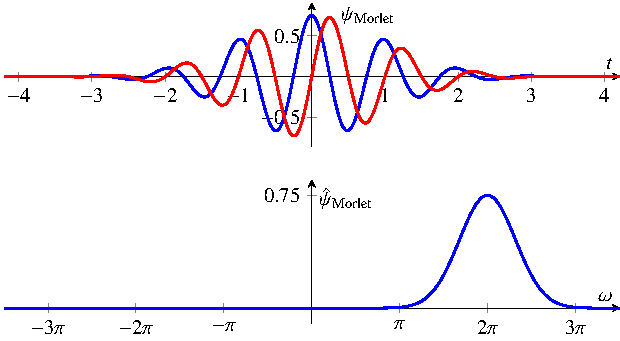
\includegraphics{papers/complex/images/morlet.pdf}
	\caption{Real- (blau) und Imaginärteil (rot) des Morlet-Wavelet für $\sigma = 2\pi$ \label{complex:morlet}}
\end{figure}

In diesem Abschnitt testen wir den Auslöschungsoperator am Gabor-Wavelet.
Wir wechseln in den Fourierbereich und nutzen aus, dass die Fouriertransformierte einer Gauss-Funktion wieder eine Gauss-Funktion ist,
\[
	\Four e^{-\alpha x^2} 
	= \frac{1}{\sqrt{2\alpha}}e^{- \frac{\omega^2}{4\alpha}},
\]
und dass die Multiplikation im Zeitbereich zur Faltung im Frequenzbereich wird.
Zudem verwenden wir die Eulerformel~\eqref{complex:euler}.
Die Fouriertransformierte des Gabor-Wavelet wird hierdurch zu

\begin{equation*}
\begin{aligned}
 \hat{\psi}_\text{Gabor}
 & = \mathcal{F}\Bigg\lbrace c_\sigma e^{-\frac{t^2}{2}}\phantom{\Bigg\rbrace}
 \cdot\; \phantom{\mathcal{F}\Bigg\lbrace}
 \Bigg(\cos\left(\sigma t\right) &&
 &&- \kappa_\sigma\Bigg) \Bigg\rbrace \\
 & = \mathcal{F}\Bigg\lbrace c_\sigma e^{-\frac{t^2}{2}} \Bigg\rbrace 
 *\: \mathcal{F}\Bigg\lbrace\Bigg( \frac12 e^{i\sigma t} &+& \frac12 e^{-i\sigma t}
 &&- \kappa_\sigma \Bigg)\Bigg\rbrace\\
 & = \phantom{\mathcal{F}\Bigg\lbrace} c_\sigma e^{- \frac{\omega^2}{2}} \phantom{\Big\rbrace}
 *\:\phantom{\mathcal{F}\Bigg\lbrace} \Bigg(
  \frac{1}{2}\delta(\omega - \sigma) &-&
  \frac{1}{2}\delta(\omega + \sigma) 
 && - \kappa_\sigma\delta(\omega)
  \Bigg).
\end{aligned}
\end{equation*}

Hierbei bezeichnet $\delta(\omega)$ die Dirac-Distribution.
Hieraus lassen sich die negative Frequenzen leicht entfernen
\footnote{
	Den Anteil von $\kappa_\sigma$ müsste man genauer betrachten.
	Durch die Faltung mit der Gauss-Funktion entstehen dadurch auch negative Frequenzen.
	Und natürlich besitzt die Exponentialfunktion keinen kompakten Träger, also entstehen auch negative Frequenzen durch die Faltung der Gauss-Ffunktion mit $\delta(\omega - \sigma)$.
	Wir begnügen uns hier für einmal mit `fast exakt'.
}.
Wir erhalten
\[
	\hat{\psi}^\ast_\text{Gabor} = 
	c_\sigma e^{- \frac{\omega^2}{2}} * (
	\!\sqrt 2 \delta(\omega - \sigma) +
	\frac{1}{\sqrt 2}\kappa_\sigma\delta(\omega) ),
\]
und durch Rücktransformation in den Zeitbereich
\[
	\psi^\ast_\text{Gabor} = c_\sigma e^{- \frac{t^2}{2}} \cdot (\!\sqrt 2 e^{i\sigma t} +	\kappa_\sigma ).
\]
Durch Skalierung der Faktoren $c_\sigma$ und $\kappa_\sigma$ werden wir die Wurzeln los und landen bei einem alten Bekannten: dem Morlet-Wavelet
\[\psi_\text{Morlet} = c_\sigma e^{- \frac{t^2}{2}} \cdot (e^{i\sigma t} + \kappa_\sigma).\]
Wir trafen es bereits in Gleichung~\eqref{cwt:morlet} als Beispiel für die CWT.
Das Morlet-Wavelet ist in Abbildung~\ref{complex:morlet} im Zeit- und Frequenzbereich dargestellt.
Auffallend ist, dass der Realteil bis auf Skalierung unverändert blieb.
Der Operator $\Ana\,$ hat also wie gewünscht das Wavelet nur minimal, respektive gar nicht verändert, sondern lediglich um einen passenden Imaginärteil ergänzt.

Abbildung~\ref{complex:morlet-ex} zeigt die beiden Wavelet-Transformationen unserer Beispiel-Signale mit dem Morlet-Wavelet.
Neu treten alle Farben auf, nicht nur jene für positive und negative Werte.
Zudem sind die Amplituden der Wavelettransformierten, also die Helligkeiten in den Bildern, nun konstant und folgen der Frequenz, statt mit dem Signal mitzuschwingen.
Ansonsten ergeben sich keine Unterschiede zu $\Wave_{\psi_\text{Gabor}}$.

\begin{figure}
	\centering
	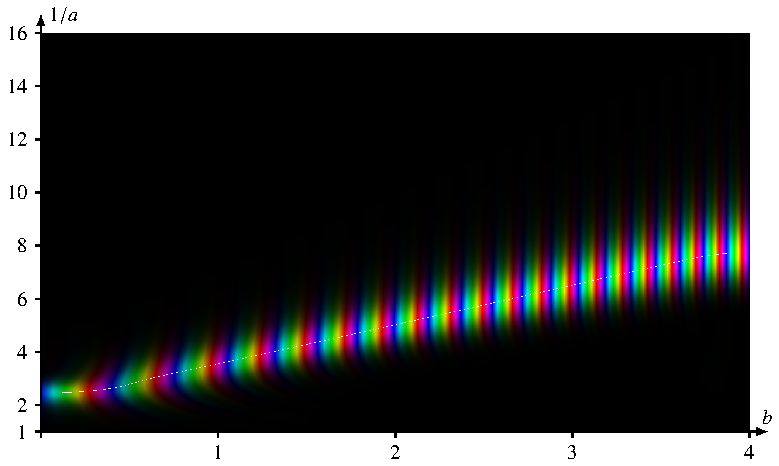
\includegraphics{papers/complex/images/chirp_morlet.pdf}
	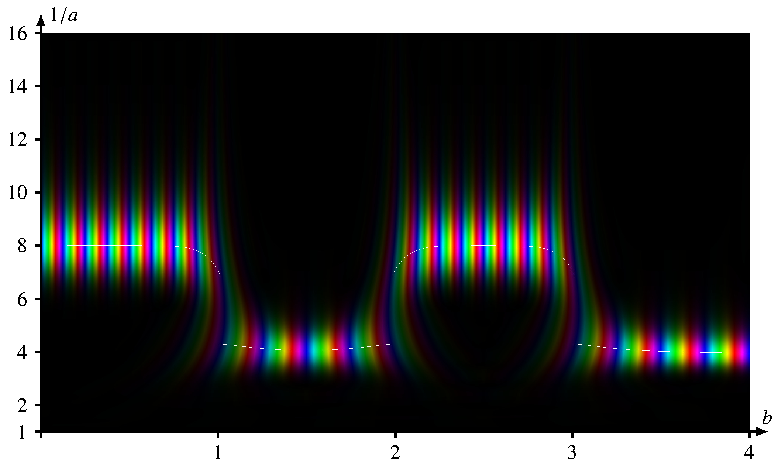
\includegraphics{papers/complex/images/square_morlet.pdf}
	\caption{Wavelet-Transformationen der beiden Beispielsignale mit dem Morlet-Wavelet. 
		Die Oszillation in der Amplitude ist verschwunden.
		Dafür sind die Skalarprodukte nun komplex, es treten alle Farben auf, nicht nur Blau und Gelb.
		Die dominante Frequenz des Morlet-Wavelet ist nahe bei $\omega_\psi \approx 1$. 
		Dadurch entspricht $1/a_\text{max}(b)$ gerade etwa der Momentanfrequenz.
		Allerdings ist die Lokalisierung in der Zeit schlechter als beim Haar-Wavelet.}
	\label{complex:morlet-ex}
\end{figure}


\section{Analytische Wavelets und Hilbert-Transformation}
\section{Analytische Wavelets}
Im vorherigen Abschnitt haben wir negative Frequenzen als Problem identifiziert.
Am Beispiel des Gabor-Wavelets suchten wir eine Lösung und fanden so das Morlet-Wavelet.
Dazu mussten alle negativen Frequenzen aus dem Spektrum des Wavelets entfernt werden.
Wie lässt sich dieses Verfahren veralgemeinern? 

Die Signaltheorie kennt genau dieses Verfahren in der Einseitenband-Modulation.
Wir entlehnen uns von dort den Begriff des \emph{analytischen Signals}\footnote{
	Der Begriff `analytisch' ist in diesem Kapitel immer im Sinne der Signaltheorie zu verstehen, also $\forall \omega < 0 \colon \hat f (\omega) = 0 $.
	Er ist nicht zu verwechseln mit der Eigenschaft analytischer Funktionen in der Analysis.
}
und defineiren analog dazu \emph{analytische Wavelets}.

\subsection{Analytische Signale und die Hilbert-Transformation}
\rhead{Hilbert-Transformation}
Bevor wir den Begriff des analytischen Signals einführen können, benötigen wir die Hilbert-Transformation
\[
\Hilb f(t) =
\frac{1}{\pi} \CH\int_{-\infty}^{\infty}\frac{f(x)}{t-x} \mathrm{d}x.
\]
Hierbei bezeichnet $\CH\int_{-\infty}^{\infty} \dots \mathrm{d}x$ den cauchysche Hauptwert des divergenten Integrals.
Diese Integral-Transformation wird uns erlauben, zu einem reellen Signal einen Imaginärteil zu finden, so dass gerade alle negativen Frequenzen im verscheinden.
Damit sind wir bereit für die Definition des analytischen Signals.

\begin{satz}
	\label{complex:analytic-signal}
	Sei $f(t) \in \mathbb{R}$ ein reelles Signal, dann heisst
	\begin{align*}
		f^\ast(t) 
		&= (1 + i\Hilb\,)f(t)
	\end{align*}
	das $f(t)$ zugeordnete \emph{analytische Signal}.
	Die Fourier-Transformierte eines analytischen Signals verschwindet für alle negativen Frequenzen.
	\[
		\forall \omega < 0 \colon \hat{f}^\ast(\omega) = 0
	\]
\end{satz}

\begin{proof}[Beweis]
	
	Die Hilbert-Transformation besitzt die Form eines Faltungs-Integrals.
	Im Frequenzbereich wird daraus eine Multiplikation.
	Es gilt mit der Signumsfunktion $\sgn(\omega)$ und der Identität
	\begin{align*}
		\Four \frac{1}{\pi t}  &= -i\sgn(\omega), \\
		\Hilb f(t) &= \frac{1}{\pi t} * f(t)\\
		\Four\Hilb f(t) &= -i\sgn(\omega) \hat{f}(\omega).
	\end{align*}
	Für die Fourier-Transformierte $\hat f^\ast(\omega)$ gilt folglich 
	\begin{align*}
		\hat{f}^\ast(\omega) 
		&= \hat{f}(\omega) - i^2\sgn(\omega)\hat{f}(\omega)\\
		&= (1 +\sgn(\omega))\hat{f}(\omega)\qedhere
	\end{align*}
\end{proof}

\begin{lemma}\label{complex:re-f-ast}
	Die Realteile von $f(t)$ und $f^\ast(t)$ sind identisch.
\end{lemma}

\begin{proof}
	Die Hilbert-Transformation ist eine reelle Integraltransformation
	\[\Hilb\,\colon\mathbb{R}\to\mathbb{R}.\]
	Folglich gilt nach Definition
	\[\Re f^\ast(t) = f(t) \quad \text{und}\quad \Im f^\ast(t) = \Hilb f(t)\qedhere\]
\end{proof}
Lemma~\ref{complex:re-f-ast} hält fest, dass wir uns durch die Hilbert-Transformation nicht zu weit vom Originalsignal entfernen.
\section{Analytische Wavelets}
Der Operator $\Ana\,$ hat den ersten Test also bestanden.
Nun möchten wir ihn noch etwas besser verstehen.
Was genau passiert eigentlich?
Ist es Zufall, dass das Morlet- und Gabor-Wavelet so ähnlich sind?
Dass der Realteil beim Morlet-Wavelet -- bis auf Skalierung -- genau dem Gabor-Wavelet entspricht?
Eine Anforderung an den Operator $\Ana\,$ war ja, dass er das Wavelet nur so wenig wie möglich ändern soll.
Beim Gabor-Wavelet hat das funktioniert.
Aber ist diese Eigenschaft im Allgemeinen erfüllt?
Diese Fragen möchten wir in diesem Abschnitt beantworten.

Im vorherigen Abschnitt haben wir negative Frequenzen als Problem identifiziert.
Wir definierten den Operator $\Ana\,$ so, dass er genau die negativen Frequenzen entfernt und dabei die Norm erhält.
Dazu wechselten wir in den Frequenzbereich, entfernten, was wir nicht wollten, und wechselten wieder zurück.

Wie lässt sich dieses Verfahren verallgemeinern? 
Ist dieses Hin- und Herwechseln tatsächlich notwendig?
Und was ist denn der Effekt im Zeitbereich?
Hierzu machen wir einen kurzen Ausflug in die Signaltheorie.
Die Theorie der analytischen Signale liefert uns die gesuchten Antworten.


\subsection{Analytische Signale und Hilbert-Transformation}
\rhead{Hilbert-Transformation}
In der Nachrichtentechnik ist Bandbreite ein beschränktes und dadurch wertvolles Gut.
Die Spektra reeller Signale weisen aber immer eine hermitesche Symmetrie auf.
Es reicht also, die Hälfte des Spektrums eines Signals zu übertragen, etwa nur die positiven Frequenzen.
In der Signaltheorie ist dieses Verfahren unter dem Namen Einseitenband-Modulation bekannt.
Ein Nebeneffekt hierbei ist, dass der Betrag des Signals gerade der Umhüllenden entspricht.
Eine Schwingung verliert damit ihre Nullstellen, ohne aber Information zu verlieren.
Genau das möchten wir von unseren Wavelets.

Ein Signal, bei welchem die negativen Frequenzen entfernt wurden, nennt man \emph{analytisches Signal}\footnote{
	Der Begriff `analytisch' ist in diesem Kapitel immer im Sinne der Signaltheorie zu verstehen, also $\forall \omega < 0 \colon \hat f (\omega) = 0 $.
	Er ist nicht zu verwechseln mit der Eigenschaft analytischer Funktionen in der Analysis.
}.
Wir werden analog dazu \emph{analytische Wavelets} definieren und zeigen, dass der Auslöschungsoperator eben solche erzeugt.
Dadurch übertragen sich die wesentlichen Eigenschaften analytischer Signale auf unsere neuen Wavelets.

Bevor wir den Begriff des analytischen Signals einführen können, benötigen wir aber die Hilbert-Transformation.
\begin{definition}
	Der Operator
 	\[
 	\Hilb\,\colon L^2(\mathbb R) \to L^2(\mathbb R)
 	~\quad~
 	f(t) \mapsto \Hilb f(t)
 	= \frac{1}{\pi} \CH\int_{-\infty}^{\infty}\frac{f(x)}{t-x} \mathrm{d}x
 	\]
 	heisst \emph{Hilbert-Transformation}.
 	Hierbei bezeichnet $\CH\int_{-\infty}^{\infty} \dots \mathrm{d}x$ den cauchyschen Hauptwert des divergenten Integrals.
\index{Hauptwert}%
\index{Cauchy-Hauptwert}%
\end{definition}

Die Hilberttransformation ist, wie die Wavelet- oder Fouriertransformation, eine Integraltransformation.
Ein wesentlicher Unterschied besteht jedoch darin, dass sie den Raum nicht wechselt.
Es ist eine Transformation aus der Zeit in die Zeit.

Nun sind wir bereit für die Definition eines analytischen Signals.
\begin{definition}
	\label{complex:analytic-signal}
	Sei $f \in L^2(\mathbb R)$ ein reelles Signal.
	Dann heisst
	\[f^\ast = (1 + i\Hilb\,)f \]
	das $f$ zugeordnete \emph{analytische Signal}.
\end{definition}
\index{analytisches Signal}
\index{Signal, analytisch}
\begin{satz}
	Ein analytisches Signal wird durch den Auslöschungsoperator erzeugt.
	\[1 + i\Hilb\, \equiv \sqrt 2 \Ana\, \Rightarrow f^\ast \equiv \sqrt 2 \Ana f\]
\end{satz}

\begin{proof}
	Der Auslöschungsoperator wechselt in den Frequenzbereich.
	Dort berechnet er die punktweise Multiplikation mit der Signumsfunktion und wechselt wieder zurück in den Zeitbereich.
	\[\Ana\, = \mathcal{F}^{-1}\frac{1+\sgn(\omega)}{\sqrt 2}\Four\]
	
	Dies ist folglich analog zur Faltung mit der inversen Fouriertransformierten der Signumsfunktion direkt im Zeitbereich,
	\[ \Ana f(t) = f(t) * \mathcal{F}^{-1}\frac{1 + \sgn(\omega)}{\sqrt 2}. \]
	
	Mit der Identität
	\[\Four\frac{1}{\pi t} = -i\sgn(\omega)\]
	so wie der Linearität der Fouriertransformation und der Faltung folgt schliesslich
	\begin{align*}
		\sqrt 2 \Ana f(t) 
		&= f(t) * \biggl(\delta(t) + \frac{i}{\pi t} \biggr)\\
		&= f(t) + \frac{i}{\pi} \CH\int_{-\infty}^{\infty} \frac{f(x)}{t - x} \,\mathrm{d}x\\
		&= (1 + i\Hilb\,) f(t)\qedhere
	\end{align*}
\end{proof}

Jetzt haben wir endlich alles zusammen, was wir für den Satz zur Ähnlichkeit brauchen.
Wir wollten ja zeigen, dass der Auslöschungsoperator das Signal nur gerade so stark verändert, wie notwendig.
Beim Morlet-Wavelet haben wir gesehen, dass er lediglich einen passenden Imaginärteil hinzufügt und das ganze so skaliert, dass die Norm erhalten bleibt.
Das stimmt für alle Wavelets.

\begin{satz}
	Sei $\psi \in L^2(\mathbb R)$ ein reelles Wavelet. Dann sind die Realteile von $\psi$ und $\Ana\psi$ bis auf Skalierung
	\[ \psi = \sqrt 2 \Re\Ana\psi\]
identisch.
\end{satz}

\begin{proof}
	Die Hilbert-Transformation ist eine reelle Integraltransformation
	\[\Hilb\,\colon L^2(\mathbb{R}) \to L^2(\mathbb{R}).\]
	Nach Definition gilt
	\[\Ana\psi = \frac{1 + i\Hilb\,}{\sqrt 2}\psi,\]
	woraus sich nun Real- und Imaginärteil direkt ablesen lassen:
	\[\Re \Ana\psi = \frac{1}{\sqrt 2}\psi \quad \text{und}\quad \Im \Ana\psi = \frac{\Hilb }{\sqrt 2}\psi.\qedhere\]
\end{proof}

Mittels Hilbert-Transformation kann also zu einem reellen Wavelet ein passender Imaginärteil gefunden werden, so dass Amplitude und Phase separiert werden können.
Wir definieren nun noch das eigentliche Objekt unserer Begierde.

\begin{satz}
	\label{complex:analytic-wavelet}
	Sei $\psi(t)$ ein reelles Wavelet. Dann ist
	\begin{equation}
	\psi^\ast = \Ana\psi
	\end{equation}
	das $\psi$ zugeordnete \emph{analytische Wavelet}.
\index{analytisches Wavelet}%
\index{Wavelet, analytisch}%
%	\footnote{Auch hierbei ist ``analytisch'' wieder im Sinne der Signaltheorie zu verstehen, also $\forall \omega < 0 \colon \hat\psi^\ast(\omega) = 0$.}
\end{satz}

Die analytischen Wavelets erben nun all die Eigenschaften analytischer Signale, welche durch den Auslöschungsoperator erzeugt werden.
Sie erhalten einen Imaginärteil, so dass sich Phase und Amplitude separieren lassen.
Analytische Wavelets eignen sich dadurch besonders gut, um periodische Anteile in einem Signal zu finden, da die Grösse des Skalarproduktes zwischen Wavelet und Signal unabhängig ist von der Phase.

Betrachten wir zum Abschluss noch beispielhaft das Haar-Wavelet.
Die Hilbert-Transformierte des Haar-Wavelets aus Definition~\ref{complex:def-haar} ist
\begin{align*}
	\Hilb \psi_{\text{Haar}}
	&= \frac{1}{\pi} \CH\int_{-\infty}^{\infty} \frac{\psi_{\text{Haar}}(x)}{t-x} dx\\
	&= \frac{1}{\sqrt2\pi}\left( \CH\int_{-0.5}^{0} \frac{1}{t-x}dx + \CH\int_{0}^{0.5} \frac{-1}{t-x}dx \right)\\
	&= \frac{1}{\sqrt2\pi} \left( -\left[\log \left|t-x\right| \right]_{-0.5}^{0} + \left[\log\left|t-x\right| \right]_{0}^{0.5} \right)\\
	&= \frac{1}{\sqrt2\pi} \left( -\log\left|t\right| + \log\left|t+0.5\right| + \log\left|t-0.5\right| - \log\left|t\right|\right)\\
	&= \frac{1}{\sqrt2\pi} \log\left|\frac{(t+0.5)(t-0.5)}{t^2}\right|
= \frac{1}{\sqrt2\pi} \log\left|\frac{t^2-0.5^2}{t^2}\right|.
\end{align*}

Daraus folgt das dem Haar-Wavelet zugeordnete analytische Wavelet
\[\psi^\ast_{\text{Haar}} = 
\frac{1}{\sqrt{2}}\biggl(\psi_{\text{Haar}} 
+ 
\frac{i}{\pi} \log\biggl|\frac{t^2-0.5^2)}{t^2}\biggr|\biggr).\]

Das analytische Haar-Wavelet ist in Abbildung~\ref{complex:ahaar} dargestellt.
Es hat keinen kompakten Träger mehr, ist jedoch noch immer gut lokalisiert in der Zeit.

Abbildung~\ref{complex:ahaar-ex} zeigt die Wavelet-Transformation mit dem analytischen Haar-Wavelet.
Die scharfe Lokalisierung in der Zeit und die schlecht Lokalisierung in der Frequenz sind wie beim reellen Haar-Wavelet. Ebenso wie die Verschiebung zwischen $1/a$ und $f$.
Wie erwartet ist jedoch die Helligkeit nun unabhängig von der Phase.

\begin{figure}
	\centering
	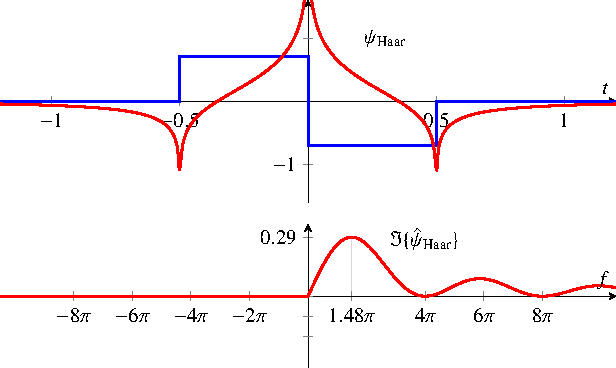
\includegraphics{papers/complex/images/ahaar.pdf}
	\caption{Das analytische Haar-Wavelet im Zeit- und Frequenzbereich.}
	\label{complex:ahaar}
\end{figure}

\begin{figure}
	\centering
	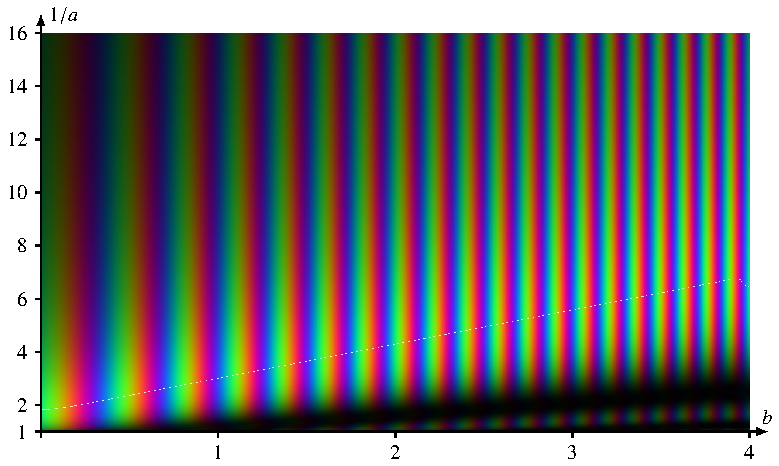
\includegraphics{papers/complex/images/chirp_ahaar.pdf}
	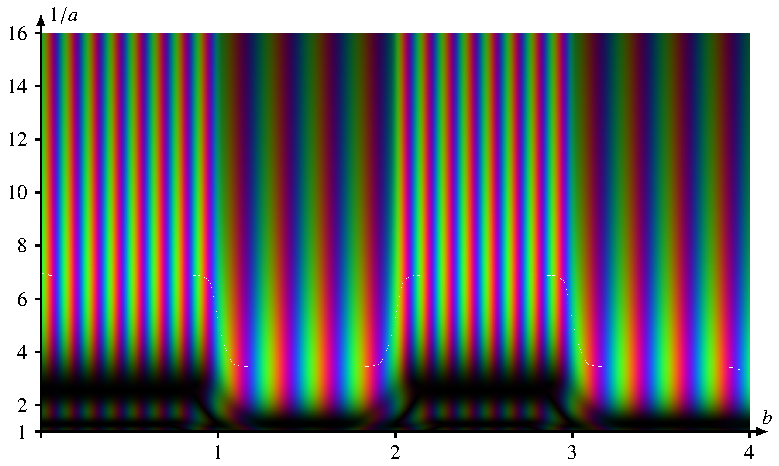
\includegraphics{papers/complex/images/square_ahaar.pdf}
	\caption{Farb-codierte Wavelet-Transformationen der beiden Beispielsignale mit dem \\ analytischen Haar-Wavelet.}
	\label{complex:ahaar-ex}
\end{figure}


\section{Zyklische Faltung, Signal-Padding und Performanz}
\rhead{Zyklische Faltung}
\label{complex:circ-conv-padding}
% TODO Padding
%% Effekt der zyklischen Faltung
%% Lösen durch padden des Signals
%%  - zero padding
%%  - padden durch spiegeln des Signals
%% Performanz-Vergleich anhand Matlab-Skript

\section{Schlussfolgerung}
\rhead{Schlussfolgerung}
%TODO Schlusswort
%% Jedes Wavelet kann in ein analytisches transformiert werden
%% Die Wavelets aus der FWT sind allerdings für die CWT ungeeignet, 
%% da sie nich in geschlossener Form im Frequenzbereich berechnet werden können
%% (Aufstellen der Faltungs-Matrix)
%% Allerdings ist das Morlet-WAvelet auch zu bevorzugen, da es die optimale 
%% Schärfe zwischen Frequenz- und Zeitauflösung beitet (Gaus\ldots)

\printbibliography[heading=subbibliography]
\end{refsection}
